% +------------------------------------------------------------------------+
% | Skin_surface_3/doc_tex/Skin_surface_3/SkinSurface3.tex
% +------------------------------------------------------------------------+
% | 2005 Nico Kruithof
% | Meshing the 3d Skin surface defined for a set of spheres.
% | 
\RCSdef{\skinSurfaceRev}{$Id$}
\RCSdefDate{\skinSurfaceDate}{$Date$}
% +------------------------------------------------------------------------+

\newcommand\ssWpoint[1]{{#1}_{(w)}}

\begin{ccTexOnly}
\begin{center}
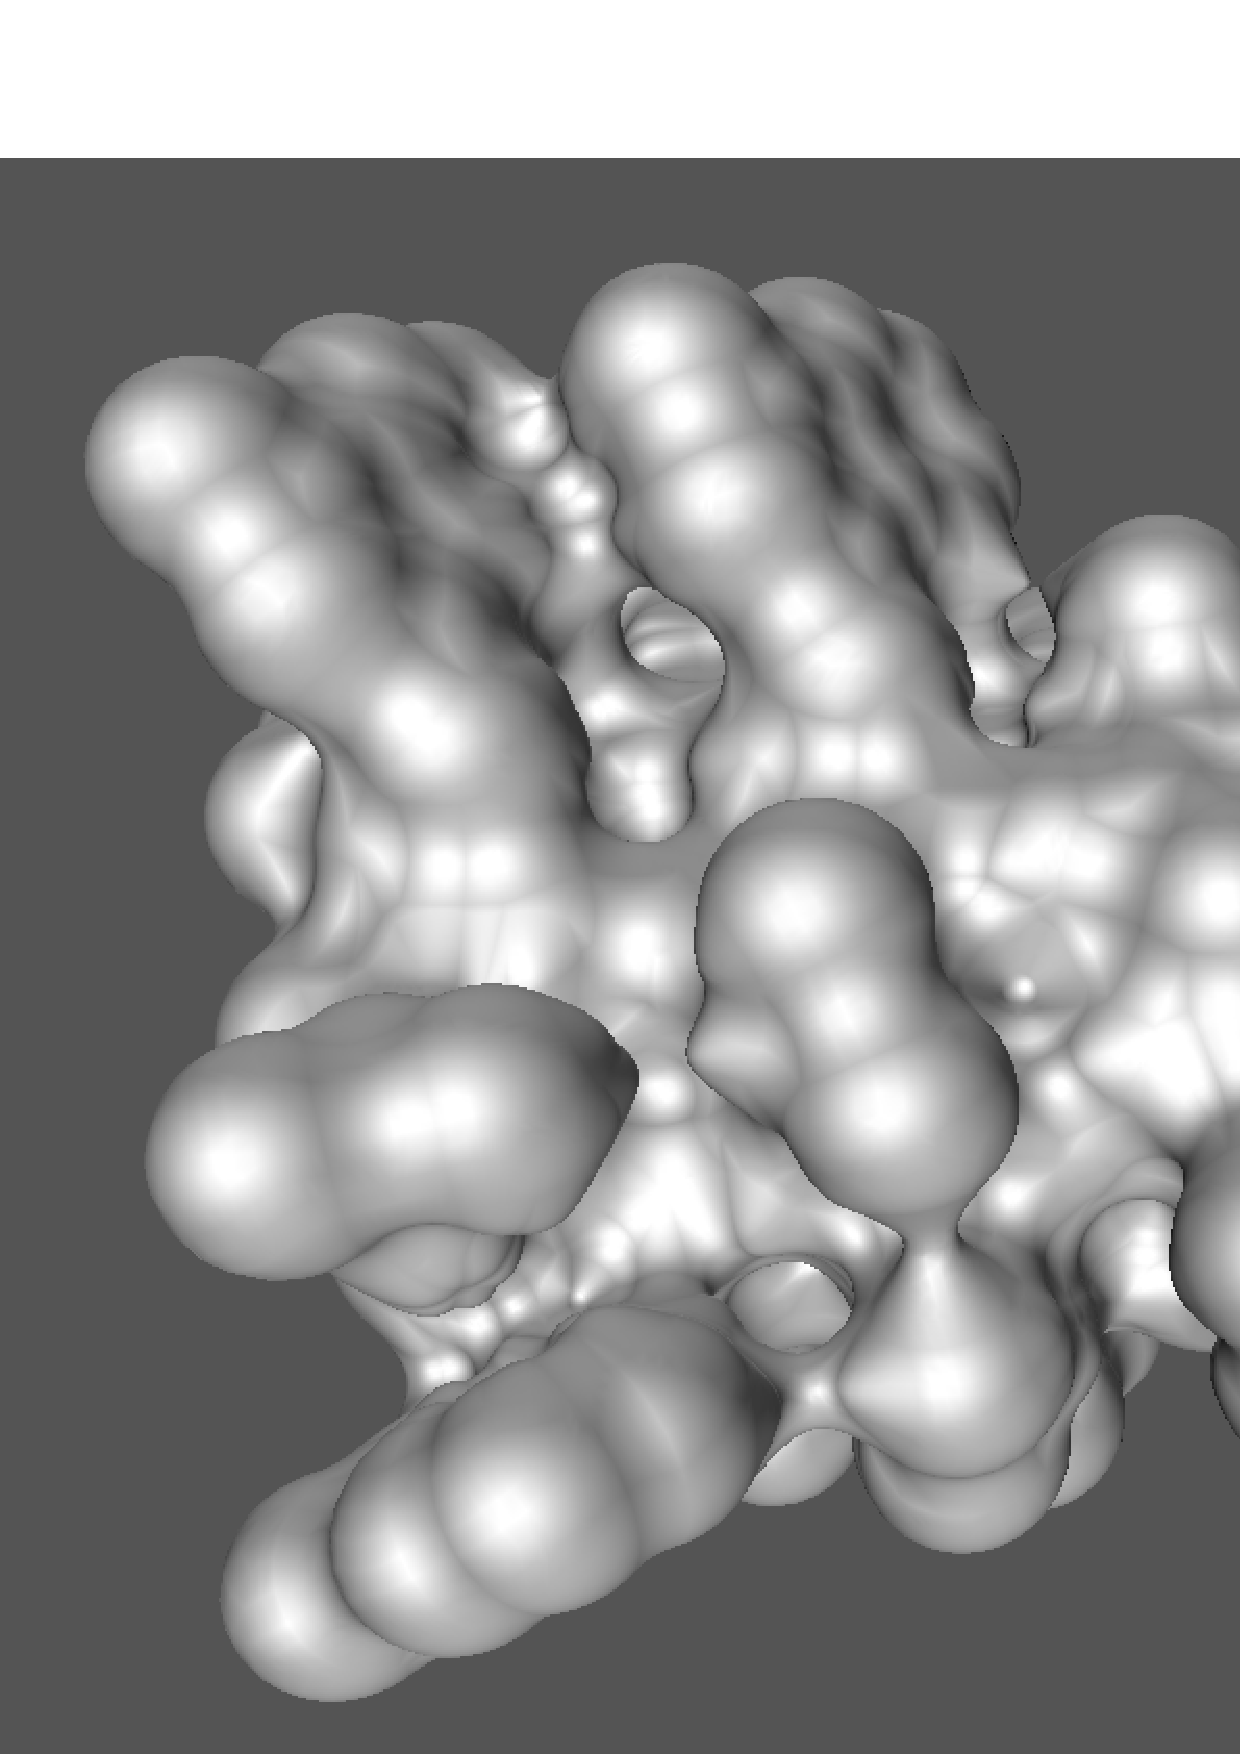
\includegraphics[width=.9\textwidth]{Skin_surface_3/molecule}
\end{center}
\end{ccTexOnly}
\begin{ccHtmlOnly}
  <center>
  <img border="0" src="./molecule.png" width="75%">
  </center>
\end{ccHtmlOnly}

% +------------------------------------------------------------------------+
\section{Introduction}
\label{sectionSkinSurfaceIntro}

Skin surfaces, introduced by Edelsbrunner in \cite{cgal:e-dssd-99},
have a rich and simple combinatorial and geometric structure that
makes them suitable for modeling large molecules in biological
computing.  Meshing such surfaces is often required for further
processing of their geometry, like in numerical simulation and
visualization.

A skin surface is defined by a set of weighted points (input balls)
and a scalar called the shrink factor. If the shrink factor is equal
to one, the surface is just the boundary of the union of the input
balls.  For a shrink factor smaller than one, the skin surface becomes
tangent continuous, due to the appearance of patches of spheres and
hyperboloids connecting the balls.

This package constructs an isotopic mesh from a set of balls and a
shrink factor using the algorithm described in
\cite{cgal:kv-mssct-05}. %It also provides an interface to the surface
%mesher presented in Chapter~\ref{chapter_SurfaceMesher} by providing a
%model of the concept \ccc{Surface_3}.

An optimized algorithm is implemented for meshing the union of a set
of balls.

\section{Definition of a skin surface}
\label{sec:skindefinition}

\begin{figure}
  \begin{ccTexOnly}
    \begin{center}
      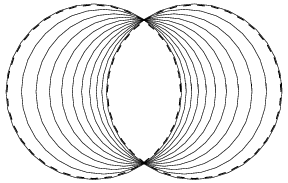
\includegraphics[width=.25\textwidth]{Skin_surface_3/convexTwoPoints}
      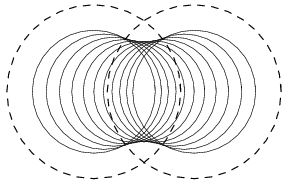
\includegraphics[width=.25\textwidth]{Skin_surface_3/skinTwoPoints}
    \end{center}
  \end{ccTexOnly}
  \begin{ccHtmlOnly}
    <center>
    <img border="0" src="./convexTwoPoints.png" align="center" alt="Convex combinations of two weighted points">
    <img border="0" src="./skinTwoPoints.png" align="center" alt="Skin
    curve of two weighted points">
    </center>
  \end{ccHtmlOnly}
  \caption{\label{fig:twoPoints} Left: Convex combinations of two
    weighted points (the two dashed circles). Right: The skin curve of
    the weighted points. The smaller circles form a subset of the
    shrunk convex hull of the input points. Its boundary forms the
    skin curve. }
\end{figure}

This section first briefly reviews skin surfaces. For a more thorough
introduction to skin surfaces, we refer to \cite{cgal:e-dssd-99} where
they were originally introduced.

A skin surface is defined in terms of a finite set of weighted points
$\ssWpoint{P}$ and a shrink factor $s$, with $0\leq s\leq 1$. A
weighted point $\ssWpoint{p}=({p},\textsc{p})\in \R^d\times\R$
corresponds to a ball with center ${p}$ and radius
$\sqrt{\textsc{p}}$. A weighted point with zero weight is called an
unweighted point. 

A pseudo distance between a weighted point $\ssWpoint{p} =
(p,\textsc{P})$ and an unweighted point $x$ is defined as
\[
\pi(\ssWpoint{p},x) = \dabs{p-x}^2 - \textsc{p},
\]
where $\dabs{p-x}$ is the Euclidean distance between $p$ and $x$.  The
ball corresponding to a weighted point $\ssWpoint{p}$ is the zero set
of $\pi(\ssWpoint{p},\cdot)$. Note that if $\textsc{p}<0$ the radius
of the ball is imaginary and the zero-set is empty.

We can take convex combinations of weighted points by taking convex
combinations of their distance functions.
%\[
%\pi(\gamma\; \ssWpoint{p} + (1-\gamma)\ssWpoint{q},x) =
%\gamma\; \pi(\ssWpoint{p},x) + (1-\gamma)\pi(\ssWpoint{q},x).
%\]
%hence the weighted point $\pi(\gamma\; \ssWpoint{p} +
%(1-\gamma)\ssWpoint{q},x)$ has center $\gamma\;p + (1-\gamma)q$ and
%weight $\gamma\;\textsc{p} + (1-\gamma)\textsc{q} +
%\gamma(1-\gamma)\dabs{p-q}$.
%
Figure~\ref{fig:twoPoints} (left) shows weighted points that
are obtained as convex combinations of the dashed circles. For further
reading on the space of circles and spheres we refer to
\cite{p-gcc-70}.

Starting from a weighted point $\ssWpoint{p}=({p},\textsc{P})$, the
shrunk weighted point $\ssWpoint{p}^s$ is obtained by taking a convex
combination with the unweighted point centered at $p$, formally
$\ssWpoint{p}^s = s \ssWpoint{p} + (1-s) p$. A simple calculation
shows that, $\ssWpoint{p}^s = ({p},s\cdot \textsc{p})$.  The set
$\ssWpoint{P}^s$ is the set obtained by shrinking every weighted point
of $\ssWpoint{P}$ by a factor $s$. The shrunk weighted points of
Figure~\ref{fig:twoPoints} (left) are shown in
Figure~\ref{fig:twoPoints} (right).

The skin surface $\mbox{skn}^{s}(\ssWpoint{P})$ associated with a set
of weighted points $\ssWpoint{P}$ is defined as the boundary of the
union of the shrunk weighted points in the convex hull of the input
weighted points:
\begin{eqnarray}
  \label{eq:defskin}
  \mbox{skn}^{s}(\ssWpoint{P}) &=& \partial{\cup(\mbox{conv} (\ssWpoint{P})^s)}.
\end{eqnarray}
%
Here $\mbox{conv}(\ssWpoint{P}) \subset \R^d\times\R$ is the convex
hull of a set of weighted points $\ssWpoint{P}$, whereas $\partial$
denotes the boundary -- in $\R^d$ -- of the union of the corresponding
set of balls. 

By definition of a skin surface, the weights of the input balls (their
radius-squared) are shrunk with a factor of $s$ and the skin surface
wraps around the shrunk input balls. In order to make the skin surface
wrap around the (unshrunk) input balls, we can first increase the
weights of the input balls by multiplying them with a factor $1/s$ and
then compute the skin surface.

%There exists a polyhedral complex that decomposes a skin surface into
%pieces quadrics. 

\section{The interface}
The interface to the skin surface package consists of two global
classes \ccc{Skin_surface_3} and \ccc{Union_of_balls_3} which are
models of the concept \ccc{Surface_3}. Further it contains two
functions to extract a mesh of the skin surface (union of balls) from
the objects of the aforementioned classes. A final function takes a
mesh and the \ccc{Skin_surface_3} (\ccc{Union_of_balls_3}) object it
is constructed from and refines the mesh. This section describes these
classes and functions in more detail.

The \ccc{Skin_surface_3} object takes an iterator range of weighted
points and a shrink factor. Optional arguments are a boolean whether
the input weighted points should be grown in such a way that the skin
surface wraps around the input balls instead of the shrunk input
balls.  The second optional argument specifies the geometric traits
class to be used.

\ccGlobalFunction{
  template <class SkinSurfaceTraits_3> 
  template < class WP_iterator >
  Skin_surface_3(
  WP_iterator begin, WP_iterator end, 
  FT shrink_factor,
  bool grow_balls = true,
  Gt gt = Gt());}

The constructor for the union of balls class is similar, except for
the missing shrink factor:

\ccGlobalFunction{
  template <class SkinSurfaceTraits_3> 
  template < class WP_iterator >
  Union_of_balls_3(
  WP_iterator begin, WP_iterator end, 
  bool grow_balls = true,
  Gt gt = Gt());}


With the \ccc{SkinSurface_3} object it is possible to generate a
coarse mesh isotopic to the skin surface. Using the function
\ccc{mesh_skin_surface_3} with signature:

\ccGlobalFunction{template <class SkinSurface_3,
                            class FT,
                            class Polyhedron>
void mesh_skin_surface_3
(SkinSurface_3 skin_surface,
 Polyhedron &p) ;}

An analogue function exists for meshing the union of a set of balls
defined by an \ccc{Union_of_balls} object:

\ccGlobalFunction{template <class UnionOfBalls_3,
                            class FT,
                            class Polyhedron>
void mesh_union_of_balls_3
(UnionOfBalls_3 union_of_balls,
 Polyhedron &p) ;}

The last function takes the (coarse) mesh and subdivides it in-situ by
applying a given number of 1-4 split operations (each triangle is
split into four sub-triangles) and moving the new vertices towards the
skin surface. If the number of iterations is not specified, one
subdivision step is done. The \ccc{SkinSurface_3} object is
needed to move the new points on the skin surface.

\ccGlobalFunction{
  template <class Polyhedron, class SkinSurface_3 >
  void subdivide_skin_surface_mesh_3 (Polyhedron &p,
  SkinSurface_3 &skinsurface,
  int iterations=1);
}

The same function can be used to subdivide the union of a set of
balls, in which case the corresponding \ccc{UnionOfBalls_3} object is
passed instead of a \ccc{SkinSurface_3} object.


%
%The class \ccc{Skin_surface_3} is both a model of the concept
%\ccc{SkinSurface_3} and the concept \ccc{Surface_3}.
%Therefore it can be used in the surface mesher described in
%Chapter~\ref{chapter_SurfaceMesher}.

\section{Timings}
The timings of the construction of the coarse mesh and the first
subdivision are given in seconds and were done on a Pentium 4, 3.5
GHz, with 1 Gb of memory.
\begin{center}
  \begin{tabular}{|l|c|c|c|}
    \hline
    Dataset & Number of weighted points & Coarse mesh & first subdivision step\\
    \hline
    \hline
    Caffeine& 23 & 0.2 & 0.05 \\
    Gramicidin A& 318 & 5 & 2\\
    \hline
  \end{tabular}
\end{center}

\section{Example programs}
\subsection{Meshing a skin surface}
The following example shows the construction of a coarse mesh of the
skin surface from an iterator range of weighted points and a shrink
factor. It first constructs an \ccc{Skin_surface_3} object from an
iterator range of weighted points and a shrink factor. From this
object, the isotopic mesh is extracted using the function
\ccc{mesh_skin_surface_3} and is stored in a \ccc{CGAL::Polyhedron}.
\ccIncludeExampleCode{Skin_surface_3/skin_surface_simple.cpp}

\subsection{Meshing and subdividing a skin surface}
This example extends the previous examples with a subdivision of the
coarse mesh to obtain a better approximation. The use of the
polyhedral items is not necessary, but gives a significant speedup.
\ccIncludeExampleCode{Skin_surface_3/skin_surface_subdiv.cpp}



